\title{Collaborative Software Development Using \R{}-Forge}
\author{Stefan Theu\ss{}l and Achim Zeileis}

\maketitle

%% Story of the article:
%% (1) Open source software (OSS) development - history, importance  _/
%%     - Apache, Linux famous examples ?TODO
%%     - Scripting languages, PHP, Perl and of course R ?TODO
%%     - software repositories: CPAN, CTAN -> CRAN ?TODO 
%% (2) collaboration and project management  _/
%%     - collaboration sites: SourceForge.net _/
%% (3) why is it important to have a central repository TODO
%%     - The Cathedral and the Bazaar TODO
%%     - large community -> better TODO
%% (4) - R-Forge  _/
%%     - explaining the basic tools  _/
%%     - R specific features  _/
%%       Package building/checking facilities
%%     - quality management through R check and tracker _/
%%     - other stuff: forums  _/

%% (5) How to forge packages on R-Forge (A day in a life of a new R
%%     package developer).
%%     - registering as a user  _/
%%     - registering a project (automatically creates SVN, a
%%       mailinglist -> managable through web interface -> click to send
%%       commit statements to this list).  _/
%%     - the svn base tree (picture of an axample tree with more
%%       packages) TODO

%% new command for R-Forge tabs
\newcommand{\tab}[1]{{\normalfont\textit{#1}}}

\section*{Introduction}

Open source software (OSS) is typically created in a decentralized
self-organizing process by a community of developers having the same
or similar interests \citep[see the famous essay by][]{forge:Raymond:1999}. 
A key factor for the success of OSS over the last two decades is the
internet: Developers who rarely meet face-to-face can employ new means
of communication, both for rapidly writing and deploying software
(in the spirit of Linus Torvald's ``release early, release often paradigm''). 
Therefore, many tools emerged that assist a collaborative software
development process, including in particular tools for source code
management (SCM) and version control.

In the \R{} world, SCM is not a new idea, in fact, the \R{}~Development
Core Team has always been using SCM tools for the \R{} sources; first by means of
Concurrent Versions System \citep[CVS, see][]{forge:Cederqvist:2006},
and then via Subversion \citep[SVN, see][]{forge:Pilato+Collins-Sussman+Fitzpatrick:2004}.
A central repository is hosted by ETH Z\"urich mainly for
managing the development of the base \R{} system. Mailing lists like
\R{}-help, \R{}-devel and many others are currently the main communication
channels in the \R{} community.

Also beyond the base system, many \R{} contributors employ
SCM tools for managing their \R{} packages, e.g., via web-based
SVN repositories like SourceForge (\url{http://SourceForge.net/})
or Google Code (\url{http://Code.Google.com/}). However, there has been
no central SCM repository providing services suited to the specific
needs of \R{} package developers.
Since early 2007, the \R{}-project offers such a central platform to the \R{}
community. \R{}-Forge (\url{http://R-Forge.R-project.org/}) provides a set
of tools for source code management and various web-based
features. It aims to provide a platform for collaborative development of
\R{} packages, \R{}-related software or further projects. \R{}-Forge is
closely related to the most famous of such platforms---the 
world's largest OSS development website---namely
\url{http://SourceForge.net/}.

%% Article Outline
The remainder of this article is organized as follows. First, we
present the core 
features that \R{}-Forge offers to the \R{} community. Second, we
give a hands-on tutorial on how users and developers can get started with 
\R{}-Forge. In particular, we illustrate how people
can register, set up new projects, use \R{}-Forge's SCM
facilities, provide their packages on \R{}-Forge, host a
project-specific website, and 
finally how package maintainers submit a package to the Comprehensive \R{}
Archive Network (CRAN, \url{http://CRAN.R-project.org/}).
Eventually, we summarize recent developments and give a brief outlook
to future work.


\section{\R{}-Forge}
%% what is R-Forge?
\R{}-Forge offers a central platform for the development of \R{}
packages, \R{}-related software and further projects. 

\R{}-Forge is based on GForge \citep{forge:copeland_et_al:2006} which is
an open source fork of the 2.61 SourceForge code maintained by Tim
Perdue, one of the original SourceForge authors. GForge has been
modified to provide additional features for the \R{} community, namely
a CRAN-style repository for hosting development releases of \R{}
packages as well as a quality management system similar to that of
CRAN.
Packages hosted on \R{}-Forge are provided in source form as well as
in binary form for Mac OS X and Windows. They can be downloaded from the
website of the corresponding project on \R{}-Forge or installed
directly in \R{}, for a package \pkg{foo}, say,
\code{install.packages("foo", repos = "http://R-Forge.R-project.org")}.

%%Tabs can be distinguished in main
%%tabs (currently Home, My Page and Project Tree) and project specific
%%tabs which are only visible when you access a project.

%% Additional Information to GForge. Since the codebase of 
%% SourceForge has not been released over a certain time the GForge
%% project was formed. 

%% Why should software developers use source code management tools?
%% FIXME: How to formulate better
%% Version control - probably the most important feature

%%Probably the most important features correspond to 3 project tabs are
%%\tab{Summary} which offers an overview of the whole project, \tab{SCM}
%%describing how people can access the source code repository and \tab{R
%%Packages} containing a list of packages available in this Project.

%% eventually include history of the development of R-Forge

On \R{}-Forge, developers organize their work
in so-called ``Projects''. Every project has various tools and
web-based features for software development, communcation and other
services. All features mentioned in the 
following sections are accessible via so-called 
``Tabs'': e.g., user accounts can be managed in the \tab{My~Page} tab or
a list of available projects can be displayed using the
\tab{Project~Tree} tab.

Since starting the platform in early 2007, more
and more interested users registered their projects on
\R{}-Forge. Now, after more than 2 years of development and testing, around
350 projects and more than 900 
users are registered on \R{}-Forge. This and the steadily growing list of
feature requests show that there is a high demand for centralized source code
management tools and for releasing prototype code frequently among the
\R{} community. %%Furthermore, based on the support e-mails we can
%%confidently say that not only developers but also users
%%(e.g., students) make use of our service.

In the next three sections, we summarize the core features of
\R{}-Forge and what \R{}-Forge offers to the \R{} community in terms
of  collaborative development of \R{}-related software projects.
%% TABS and projects

\subsection{Source Code Management}

When carrying out software projects, source files change over time,
new files get created and old files deleted. Typically, several authors
work on several computers on the same and/or different files and keeping
track of every change can become a tedious task. In the open source
community, the general solution to this problem is to use version
control, typically 
provided by the majority of SCM tools. For this reason \R{}-Forge
utilizes SVN to facilitate the developer's work when creating
software.

A central repository ensures that the developer
has always access to the current version of the project's source
code. Any of the authorized collaborators can ``checkout''
(i.e., download) or ``update'' the project
file structure, make the necessary changes or additions, delete
files from the current revision and finally ``commit'' changes or
additions to the repository. More than
that, SVN keeps track of the complete history of the project file
structure. At any point in the development stage it is possible to go
back to any previous stage in the history to inspect and restore old
files. This is called version control as every stage automatically is
assigned a unique version number which increases over time. 

%% SCM on R-Forge
On \R{}-Forge such a version-controlled repository is automatically
created for each project. To get started, the project members just
have to install the client of their choice (e.g., Tortoise SVN on
Windows or svnX on 
Mac OS X) and check out the repository. In addition to the inherent
backup of every version within the repository a backup of the whole
repository is generated daily. 

%% Rights management on R-Forge
A rights management system assures that, by default, anonymous users
have read access and developers have write access to the data associated with 
a certain project on \R{}-Forge. More precisely, registered users can
be granted one of several roles: e.g., the ``Administrator'' has
all rights including the right to 
add new users to the project or release packages directly to CRAN.
He/she is usually the package 
maintainer, the project leader or has registered the project originally.
Other members of a project typically have either the role ``Senior 
Developer'' or ``Junior Developer'' which both have permission to
commit to the project SVN repository and examine the log files in the 
\tab{R Packages} tab (the differences between the two
roles are subtle, e.g., senior developers additionally have administrative
privileges in several places in the project).  
When we speak of developers in subsequent sections we refer to project
members having the rights at least of a junior developer.


\subsection{Release and Quality Management}
\label{sec:release_and_quality_management}

%% Quality Management and bug/support/feature tracker
Development versions of a software project are typically
prototypes and are subject to many changes. Thus, \R{}-Forge offers
two tools which assist the developers in improving the quality of
their source code.

First, it offers a quality management system similar to 
that of CRAN. Packages on \R{}-Forge are checked in a
standardized way on different platforms based on
\code{R~CMD~check} at least once daily. The resulting log files can be
examined by the project developers so that they can improve
the package to pass all tests on \R{}-Forge and subsequently on CRAN.

Second, bug tracking systems allow users to notify
package authors about problems they encounter. In the spirit of
OSS---given enough eyeballs, all bugs are shallow
\citep{forge:Raymond:1999}---peer code review leads to an 
overall improvement of the quality of software projects.

\subsection{Additional Features}

A number of further tools, of increased interest for larger
projects, help developers to coordinate their work and to communicate
with their user base. These tools include:

\begin{itemize}
\item Project websites: Developers may present their work
  on a subdomain of \R{}-Forge, e.g.,
  \url{http://foo.R-Forge.R-project.org/}, or via a link to an
  external website.
%% checked out hourly from ``www'' directory of the
%%project's repository.
\item Mailing lists: By default a list
  \code{foo-commits@\\lists.R-Forge.R-project.org} is automatically
  created for each project. Additional mailing lists can be
  set up easily.
\item Project categorization: Administrators may categorize their
  project in several so-called ``Trove Categories'' in the \tab{Admin}
  tab of their project (under \tab{Trove Categorization}). For each
  category three different items can be selected. This enables users
  to quickly find what they are looking for using the \tab{Project Tree}
  tab.
\item News: Announcements and other information related to a project
  can be put on the project summary page as well as on the 
  home page of \R{}-Forge. The latter needs approval by one of the \R{}-Forge
  administrators. All items are available as RSS feeds.
\item Forums: Discussion forums can be set up separately by the
  project administrators.%% are places to discuss certain topics 
\end{itemize}

\section{How to Get Started}
%%A small guide through R-Forge---detailed explanation in user's manual 
This section is intended to be a hands-on tutorial for new
users. Depending on the familiarity with the systems/tools involved
the instructions might be somewhat brief. In case of problems we
recommend to consult the user's manual \citep{forge:usermanual:2008}
which contains detailed step-by-step instructions.

\setkeys{Gin}{width=0.95\textwidth}
\begin{figure*}[th]
\centering
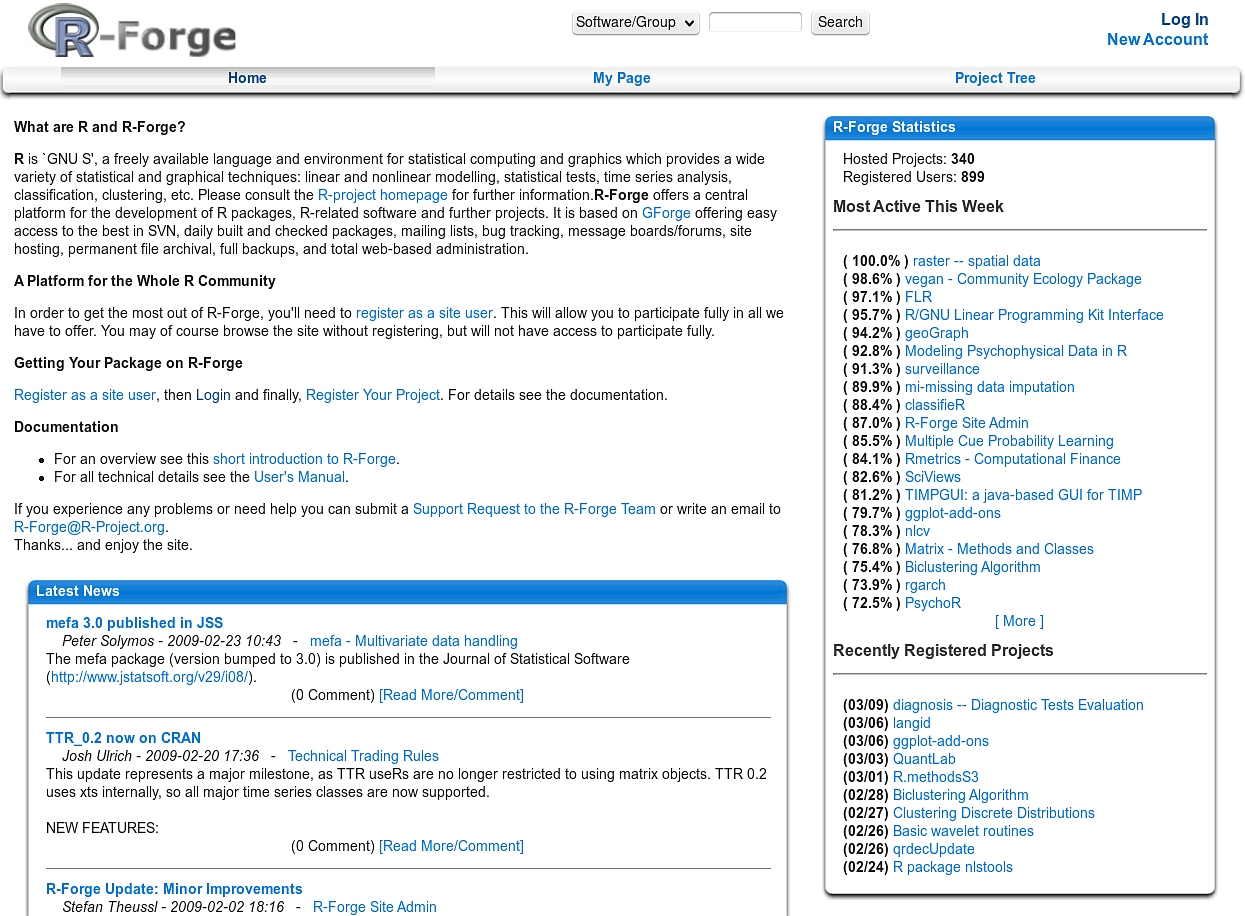
\includegraphics{rforge_main_snapshot_modified.png}
\caption{Home page of \R{}-Forge on 2009-03-10}
\label{fig:home_page}
\end{figure*}

When accessing the URL \url{http://R-Forge.R-project.org/} the home
page is presented (see Figure~\ref{fig:home_page}). Here one can

\begin{itemize}
\item login,
\item register a user or a project,
\item download the documentation,
\item examine the latest news and changes,
\item go to a specific project website either by searching for available
  projects (top middle of the page), by clicking on one of the projects
  listed on the right, or by going through the listing in
  the \tab{Project Tree} tab.
%% some \R{}-Forge specific statistics (how many projects/users
%%  are currently registered on \R{}-Forge, project activity percentages,
%%  etc.).
\end{itemize}

Registered users can access their personal
page via the tab named \tab{My Page}. Figure~\ref{fig:my_page} shows
the personal page of the first author.

\setkeys{Gin}{width=0.95\textwidth}
\begin{figure*}[th]
\centering
\includegraphics{rforge_my_page_snapshot.png}
\caption{The \tab{My Page} tab of the first author}
\label{fig:my_page}
\end{figure*}

\subsection{Registering as a New User}

For using \R{}-Forge as a developer, one has
to register as a site user. A link on the main web site called
\tab{New Account} on the top right of the home page leads to the
corresponding registration form.

After submitting the completed form, an e-mail is sent to the given
address containing a link for activating the account. Subsequently,
all \R{}-Forge features, including joining existing or creating
new projects, are available to logged-in users.

\subsection{Registering a Project}

There are two possibilities to register a project: Clicking on
\tab{Register Your Project} on the home page or by going to the 
\tab{My Page} tab and clicking on \tab{Register Project}~(see
Figure~\ref{fig:my_page} below the main tabs). Both links lead to a
form which has to be filled out in order to finish the registration
process. In the text field ``Project Public Description'' the
registrant is supposed to enter a short and concise description of the
project. This text and the ``Project Full Name'' will be shown in
several places on \R{}-Forge (see e.g., Figure~\ref{fig:home_page}). The text 
entered in the field ``Project Purpose And Summarization'' is an
additional information for the \R{}-Forge administrators, inspected
for approval. ``Project Unix
Name'' refers to the name which 
uniquely determines the project. In case of a project that contains a
single \R{} package, the project Unix name typically corresponds to
the package name (in its lower-case version). Restrictions according to
the Unix file system convention force Unix names to be in lower case
(and will be converted automatically if they are typed in upper case).

After the completed form was submitted, the project has to be approved
by the \R{}-Forge administrators and a confirmation e-mail is sent to the
registrant upon approval. After that, the registrant automatically
becomes the project administrator and the standardized web area of the
project (\code{http://R-Forge.R-project.org/projects/foo/}) is
immediately available on \R{}-Forge. 
This web area includes a \tab{Summary} page, an \tab{Admin} tab
visible only to the project administrators, and various other tabs
depending on the features enabled for this project in the \tab{Admin}
tab. To present the new project to a broader community the name of the
project additionally is promoted on the home page under ``Recently
Registered Projects'' (see Figure~\ref{fig:home_page}).

Furthermore, within an hour after approval a default mailing list and
the project's SVN repository containing a \file{README} file and two
pre-defined directories called \file{pkg} and \file{www} are created. 
The content in these directories is used by the \R{}-Forge server
for creating \R{} packages and a project website, respectively.


\subsection{SCM and \R{} Packages}

The first step after creation of a project is typically to start
generation of content for one (or more) \R{} package(s) in the \file{pkg}
directory. Developers can either start committing changes via SVN as usual
or---if the package is already version-controlled somewhere else---the
corresponding parts of the repository including the history can be 
migrated to \R{}-Forge (see Section~6 of the user's manual).

The \tab{SCM} tab of a project explains how the corresponding SVN
repository located at \code{svn://svn.R-Forge.R-project.org/svnroot/foo}
can be checked out. From
this URL the sources are checked out either 
anonymously without write permission (enabled by default) or as
developer using an encrypted authentication method, namely secure
shell (\code{ssh}). Via this secure protocol (\code{svn+ssh://}
followed by the registered user name) developers have full access to the
repository. Typically, the developer is being authenticated via the
registered password but it is also possible to upload a secure shell
key (updated hourly) to make use of public/private key
authentication. Section~3.2 of the user's manual explains this process
in more detail.

To make use of the package builds and checks
the package source code has to be put into the \file{pkg} directory
of the repository (i.e., \file{pkg/DESCRIPTION},
\file{pkg/R}, \file{pkg/man}, etc.) or, alternatively, a 
subdirectory of \file{pkg}. The latter structure allows to
have more than one package in a single project, e.g., if
a project consists of the packages \code{foo} and \code{bar}, then the
source code is located in \file{pkg/foo} and \file{pkg/bar},
respectively.

\R{}-Forge automatically examines the \file{pkg} directory of
every repository and builds the package sources as well as the package
binaries on a daily basis for Mac OS X and Windows (if applicable). The
package builds 
are provided in the \tab{R Packages} tab (see
Figure~\ref{fig:rpackages_tab}) for download or can be 
installed directly in \R{} using 
\code{install.packages("foo",
  repos="http://R-Forge.R-project.org")}. Furthermore, in the \tab{R
  Packages} tab developers can examine logs of the build and check
process on different platforms. 

To release a package to CRAN the project administrator clicks on
\tab{Submit this package to CRAN} in the \tab{R Packages} tab. Upon
confirmation, a message will be sent to \email{CRAN@R-project.org} and
the latest successfully built source package (the \file{.tar.gz}) is
automatically 
copied to \url{ftp://CRAN.R-project.org/incoming/}. Note that packages
are built once daily, i.e., the latest source package does not
include more recent code committed to the SVN repository. 

Figure~\ref{fig:rpackages_tab} shows the \tab{R Packages} tab of the
tm project (\url{http://R-Forge.R-project.org/projects/tm/}) as one of
the project administrators would see it. Depending on whether you are
a member of the project or not and your rights you will see only parts
of the information provided for each package.

\setkeys{Gin}{width=0.95\textwidth}
\begin{figure*}[th]
\centering
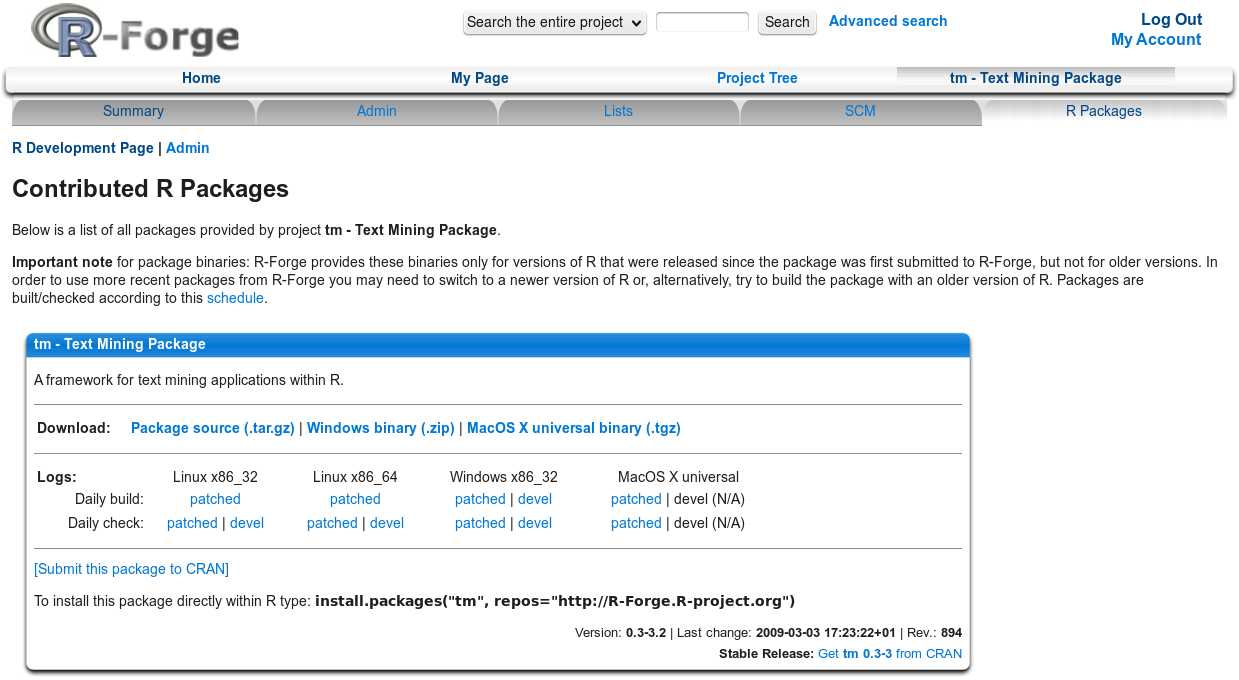
\includegraphics{rforge_tm_packages_developer_snapshot.png}
\caption{\tab{R Packages} tab of the tm project}
\label{fig:rpackages_tab}
\end{figure*}

\subsection{Further Steps}

A customized project website, accessible through
\url{http://foo.R-Forge.R-project.org/} where \code{foo} 
corresponds to the unix name of the project, is managed via the
\file{www} directory. The website gets updated every hour. 

The changes made to the project can be examined by entering the
corresponding standardized web area. On entry, the \tab{Summary}
page is shown. Here, one can 

\begin{itemize}
\item examine the details about the project including a short
  description and a listing of the administrators and developers,
\item follow a link leading to the project homepage,
\item examine the latest news announcements (if available),
\item go to other sections of the project like
  \tab{Forums}, \tab{Tracker},
   \tab{Lists}, \tab{R Packages}, etc.
\item follow the download link leading directly to the available
  packages of the project (i.e., the \tab{R Packages} tab).
\end{itemize}

Furthermore, meta-information about a project can be supplied in
the \tab{Admin} tab via so-called ``Trove Categorization''. 


\section*{Recent and Future Developments}

In this section, we briefly summarize the major changes and updates to
the \R{}-Forge system during the last months and give an outlook to
future developments. 

Recently added features and major changes include:

\begin{itemize}
\item New defaults for freshly registered projects: Only the tabs
  \tab{Lists}, \tab{SCM} and \tab{R~packages} are enabled
  initially. \tab{Forums}, \tab{Tracker} and \tab{News}
  can be activated separately (in order not to overwhelm
  new users with too many features) using \tab{Edit Public Info} in
  the \tab{Admin} tab of the project. Experienced users can decide
  which features they want and activate them.
\item An enhanced structure in the SVN repository allowing multiple
  packages in a single project (see above).
\item The \R{} package \pkg{RForgeTools} \citep{forge:theussl:2008}
  contains platform-independent package
  building and quality management code used on the \R{}-Forge servers.
\item A modified \tab{News} submit page offering two types of
  submissions: project-specific and global news. The latter
  need an approval by one of the \R{}-Forge administrators (default:
  project-only submission).
\item Circulation of SVN commit messages can be enabled in the
  \tab{SCM Admin} tab by project administrators. The mailing list mentioned in
  the text field is used for delivering the SVN commit messages
  (default: off). 
\item Mailing list search facilities provided by the Swish-e engine
  which can be accessed via the \tab{List} tab (private lists
  are not included in the search index).

\end{itemize}

Further features and improvements which are currently on the wishlist
or under development include 

\begin{itemize}
\item a Wiki,
\item task management facilities,
\item a re-organized tracker more compatible with \R{} package
  development and,
\item an update of the underlying GForge system to its successor
  FusionForge~(\url{http://FusionForge.org/}).
\end{itemize}

For suggestions, problems, feature requests, and other questions regarding
\R{}-Forge please contact \email{R-Forge@R-project.org}.

\section{Acknowledgments}

Setting up this project would not have been possible without Douglas
Bates and the University of Wisconsin as they provided us with a
server for hosting this platform. Furthermore, 
the authors would like to thank the Computer Center 
of the Wirtschaftsuniversit\"at Wien for
their support and for providing us with additional hardware as well as a
professional server infrastructure.

\bibliography{R-Forge}
